\section{Preliminary}
\subsection{3D Gaussian splatting}
\label{sec:related_work}
Distinct from the widely adopted
Neural Radiance Field, 3D Gaussian Splatting is an explicit 3D scene representation in the form of point clouds, where Gaussian splats are utilized to represent the structure of the scene. In this representation, every Gaussian splat $G$ is defined by a full 3D covariance matrix $\Sigma$ as well as the center (mean) $x \in R^3$.
\begin{align}
    G(x)=e^{-1/2(x)^T\Sigma^{-1}(x)} \
\end{align}
The covariance matrix $\Sigma$ of a 3D Gaussian splat can be likened to characterizing the shape of an ellipsoid. Therefore, we can describe it using a rotation matrix R and a scale matrix S and independently optimize of both them. 
\begin{align}
    \Sigma=RSS^TR^T
\end{align}
 To project our 3D Gaussian splats to 2D for rendering, the method of splatting  is utilized for positioning the Gaussian splats
on the camera planes:
\begin{align}
    \Sigma'=JW\Sigma W^TJ^T
\end{align}
Where J is the Jacobian of the affine approximation of the projective transformation and W is the viewing transformation.
Following this, the pixel color is obtained by alpha-blending N sequentially layered 2D Gaussian splats from front to back:
\begin{align}
    C=\sum_{\substack{i\in N}}c_{i}\alpha_{i}\prod_{j=1}^{i-1}(1-\alpha_{j}) \label{point rendering}
\end{align}
Where $c_{i}$ is the color of each point and $\alpha_{i}$
is given by evaluating a 2D Gaussian with covariance $\Sigma$ multiplied with a learned per-point opacity.
\subsection{Precompute Radiance Transfer}
According to \cite{kajiya1986rendering}, the outgoing radiance $L_o$ at a point $x$ with normal $n$ observed by the camera in direction $\omega_o$ is given by the Rendering Equation:
\begin{align}
    L_o(\omega_o,x)=L_e+\int_{\Omega}f(x,\omega_i,\omega_o)L_i(\omega_i,x)(\omega_i,n)V(\omega_i,x)d\omega_i  \label{rendering equation}
\end{align}
where $L_i$ corresponds to the incident light coming from direction $\omega_i$, and $f(x,\omega_i,\omega_o)$ represents the Bidirectional Reflectance Distribution Function (BRDF) properties of the point corresponding to $\omega_i$ and outgoing direction $\omega_o$. If we assume that objects in the scene do not have self-emission. Further, we have:
 \begin{align}
    L_o(\omega_o,x)=\int_{\Omega}T(x,\omega_i,\omega_o)L_i(\omega_i\cdot x)d\omega_i \label{rendering transfer equation}
\end{align}  
where 
\begin{align}
    T(x,\omega_i,\omega_o)=f(x,\omega_i,\omega_o)(\omega_i \cdot n)V(\omega_i,x)
\end{align} 
corresponds to the radiance transfer.
Our goal is to precompute incident light $L_i$ and radiance transfer $T$ and project them into SH domain. 
According to \cite{sloan2002precomputed}, any function $F(s)$ defined on the sphere $S$ can be represented as a set of SH basis functions:
\begin{align}
    F(s)=\sum_{l=0}^{n-1}\sum_{m=-l}^{l}f_l^mY_l^m(s)
\end{align}
where n denotes the degree of SH and $Y_l^m(s)$ is a set of real basis of SH.
Because the SH basis is orthonormal, the scalar function $F$ can be projected into its coefficients via the integral:
\begin{align}
    f_l^m=\int F(s)Y_l^m(s)ds \label{sh_jifen}
\end{align}  
Then, $L_i(\omega_i)$ at $x$ defined on $\omega_i$ can be represented as:
\begin{align}
    L_i(\omega_i)=\sum_{l=0}^{n-1}\sum_{m=-l}^{l}l_l^mY_l^m(\omega_i)=\sum_{j=1}^{n^2}l_jY_j(\omega_i) \label{sh2}
\end{align}
and for diffuse cases, $f(x,\omega_i,\omega_o)=\rho/\pi$ which is not related to $\omega_o$, we have: 
\begin{align}
    T_i(\omega)=\sum_{l=0}^{n-1}\sum_{m=-l}^{l}t_l^mY_l^m(\omega_i)=\sum_{j=1}^{n^2}t_jY_j(\omega_i) \label{prt sh}
\end{align}
Because $T$ is also defined only on $\omega_i$.
Equation \ref{rendering equation} can be written as:
\begin{align}
    L_o(x)=\sum_{p=1}^{n^2}\sum_{q=1}^{n^2}l_pt_q\int_{\Omega}Y_p(\omega_i)Y_q(\omega_i)d\omega_i \label{prt}
\end{align}
Considering:
\begin{align}
    \int_{\Omega}Y_p(\omega_i)Y_q(\omega_i)d\omega_i = 
        \begin{cases}
        1 & \text{if } q=p \\
        0 & \text{otherwise}
        \end{cases} \label{eq:sx}
\end{align}
Then equation \ref{prt} can be written as:
\begin{align}
    L_o(x)=\sum_{i=0}^{n^2}l_it_i=\Vec{L} \cdot \Vec{T}
\end{align}
where $\Vec{T}$=\{$t_1$,\dots,$t_{n^2}$\} and $\Vec{L}$=\{$l_1$,\dots,$l_{n^2}$\}. In summary, we can project the lighting and radiance transfer to the basis to obtain $\Vec{L}$ and $\Vec{T}$. Rendering at each point is reduced to a dot product. For glossy cases, light transport will be obtained as a transfer matrix. Please refer to sec \ref{4.5} and supplementary for more details.
\begin{figure*}[htbp]
\centering
  \vspace{-0.3cm}
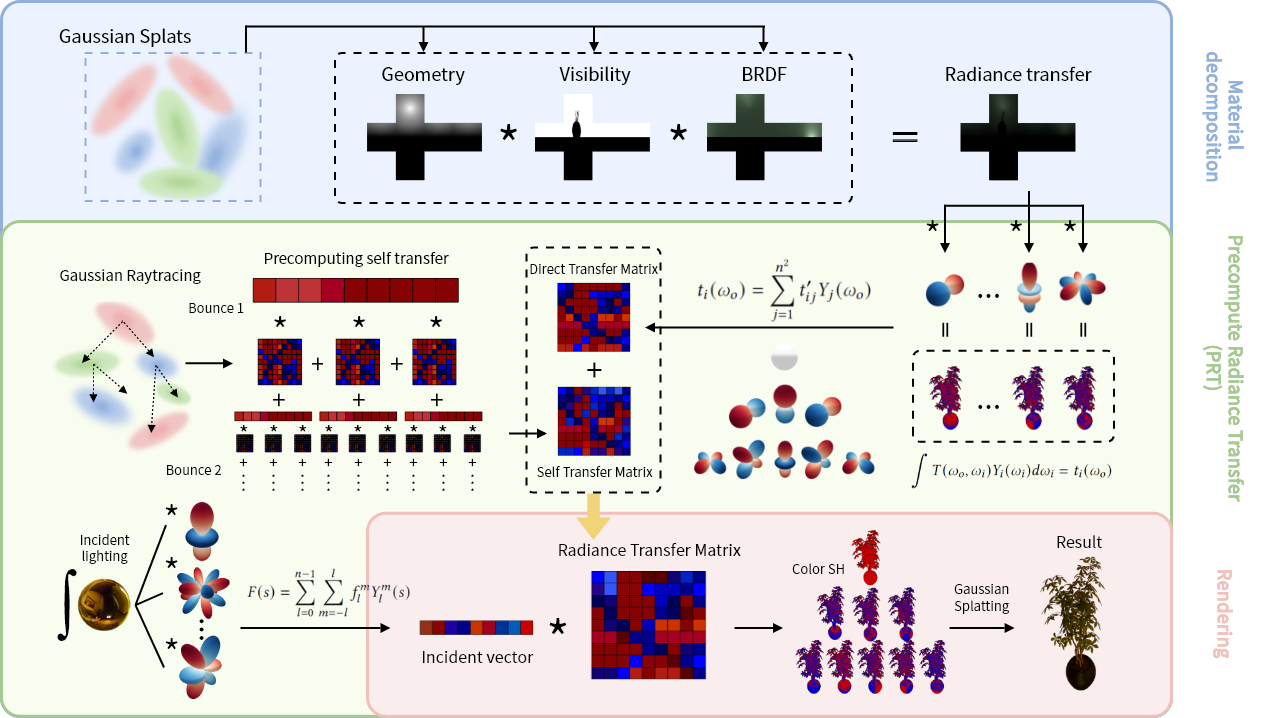
\includegraphics[width=\linewidth]{figures/pipeline3.png}
\caption{ The proposed rendering pipeline. Starting with a collection of 3D Gaussian splats that embody geometry, visibility, and BRDF attributes along with incident lighting, we first compute the radiance transfer for every Gaussian splat by executing equation \ref{glossy transfer}, the direct transfer matrix by equation \ref{glossy prt} and the incident vector by equation \ref{sh2}. Following this, we conduct one-bounce 3D Gaussian ray tracing (Sec 4.4) to get the index matrix and precompute self-transfer for every Gaussian splat recursively to estimate indirect illumination based on the index matrix. Finally, we conduct a straightforward dot product between the radiance transfer matrix and incident vector in the spherical harmonics domain and compute the final rendering result with Gaussian splatting. }\label{pipeline}
  \vspace{-0.6cm}
\end{figure*}